% !TeX root = Thesis.tex

\begin{figure}[ht]
    \centering
    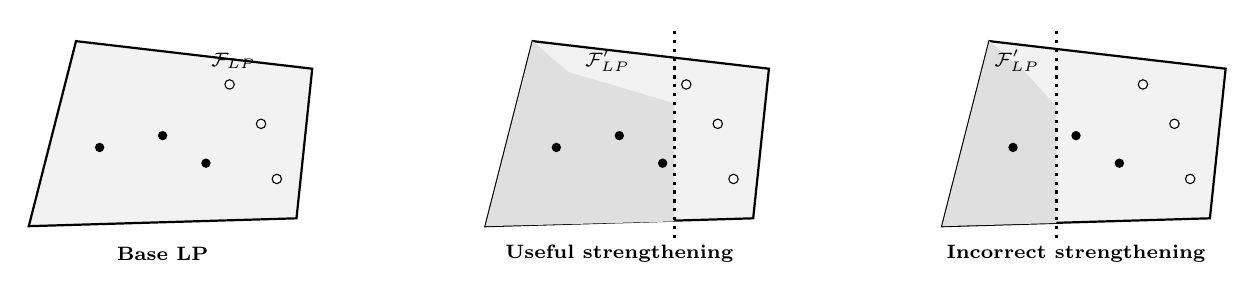
\begin{tikzpicture}[
        >=stealth,
        every node/.style={font=\scriptsize},
        feasible/.style={circle,fill=black,inner sep=1.2pt},
        fractional/.style={circle,fill=white,draw=black,inner sep=1.2pt}
    ]

    % Base LP
    \begin{scope}
        \draw[thick,fill=gray!10]
            (-1.7,-0.95) -- (1.7,-0.85) -- (1.9,1.05) -- (-1.1,1.4) -- cycle;

        \node[feasible] at (-0.8,0.05) {};
        \node[feasible] at (0.0,0.2) {};
        \node[feasible] at (0.55,-0.15) {};

        \node[fractional] at (0.85,0.85) {};
        \node[fractional] at (1.25,0.35) {};
        \node[fractional] at (1.45,-0.35) {};

        \node at (0.9,1.15) {$\mathcal{F}_{LP}$};

        \node[font=\scriptsize\bfseries] at (0,-1.3)
            {Base LP};
    \end{scope}


    % Useful strengthening
    \begin{scope}[xshift=5.8cm]
        % Original LP region
        \draw[thick,fill=gray!10]
            (-1.7,-0.95) -- (1.7,-0.85) -- (1.9,1.05) -- (-1.1,1.4) -- cycle;

        % New feasible region
        \fill[gray!25]
            (-1.7,-0.95) -- (0.7,-0.89) -- (0.7,0.61)
            -- (-0.65,1.01) -- (-1.1,1.4) -- cycle;

        % Added vertical constraint
        \draw[dotted,very thick] (0.7,-1.1) -- (0.7,1.55);

        % Same points
        \node[feasible] at (-0.8,0.05) {};
        \node[feasible] at (0.0,0.2) {};
        \node[feasible] at (0.55,-0.15) {};

        \node[fractional] at (0.85,0.85) {};
        \node[fractional] at (1.25,0.35) {};
        \node[fractional] at (1.45,-0.35) {};

        \node at (-0.15,1.15) {$\mathcal{F}_{LP}'$};

        \node[font=\scriptsize\bfseries] at (0,-1.3)
            {Useful strengthening};
    \end{scope}


    % Incorrect strengthening
    \begin{scope}[xshift=11.6cm]
        % Original LP region
        \draw[thick,fill=gray!10]
            (-1.7,-0.95) -- (1.7,-0.85) -- (1.9,1.05) -- (-1.1,1.4) -- cycle;

        % New feasible region
        \fill[gray!25]
            (-1.7,-0.95) -- (-0.25,-0.91) -- (-0.25,0.57)
            -- (-0.65,1.01) -- (-1.1,1.4) -- cycle;

        % Added vertical constraint
        \draw[dotted,very thick] (-0.25,-1.1) -- (-0.25,1.55);

        % Same points
        \node[feasible] at (-0.8,0.05) {};
        \node[feasible] at (0.0,0.2) {};
        \node[feasible] at (0.55,-0.15) {};

        \node[fractional] at (0.85,0.85) {};
        \node[fractional] at (1.25,0.35) {};
        \node[fractional] at (1.45,-0.35) {};

        \node at (-0.75,1.15) {$\mathcal{F}_{LP}'$};

        \node[font=\scriptsize\bfseries] at (0,-1.3)
            {Incorrect strengthening};
    \end{scope}

    \end{tikzpicture}
    \caption{Strengthening the linear program with an additional constraint. Each panel shows the same feasible region and candidate solutions, with valid roots represented by filled black dots and invalid roots by unfilled white dots. The position of the additional constraint determines which solutions remain feasible. A suitable constraint eliminates fractional solutions while retaining all valid integer solutions, whereas an overly restrictive constraint also excludes valid integer solutions.}
    \label{fig::LP_strengthening}
\end{figure}